\begin{example}[Advection-diffusion 2D]
\label{ex:quart2}
Based on Example 2 \cite{Antonietti2013},
in $\Omega = \langle 0, 1 \rangle^2$ we will again solve equation \eqref{eq:ex_advdiff}
%\begin{equation}
%	\pdiff{u}{x} + \pdiff{u}{y} - D \cdot \left( \pdiff{^2 u}{x^2} + \pdiff{^2 
%	u}{y^2} \right) = g
%\end{equation}
%i.e
%\begin{equation}
%	\vec{a} \cdot \nabla u - D \Delta u = g
%\end{equation}
%where $\vec{a} = [1, 1]^T$ is advection velocity and $D$ is diffusion 
%coefficient and $g$ is a source function. 
We setup boundary condition and source function in such way that the exact 
solution $u_{exact}$ is
\begin{equation}
	u_{exact} =  -\arctan\left(\frac{4 \, {\left(2 \, x - 1\right)}^{2} + 4 \, {\left(2 
	\, y - 1\right)}^{2} - 
	1}{16 \, \sqrt{\mathit{D}}}\right).
\end{equation}
We omit analytical forms of $g$ and boundary conditions for brevity, they can be found in 
the code.
Different values of coefficient $C_w$ in penalty term yield different 
convergence behavior as demonstrated in Figure \ref{fig:conv_qart2} and 
\Cref{fig:orders_quarteroni2}.
\end{example}

\begin{figure}[h!]
\centering
\begin{tabular}{p{0.5\textwidth} p{0.5\textwidth}}
	\vspace{0pt} 
	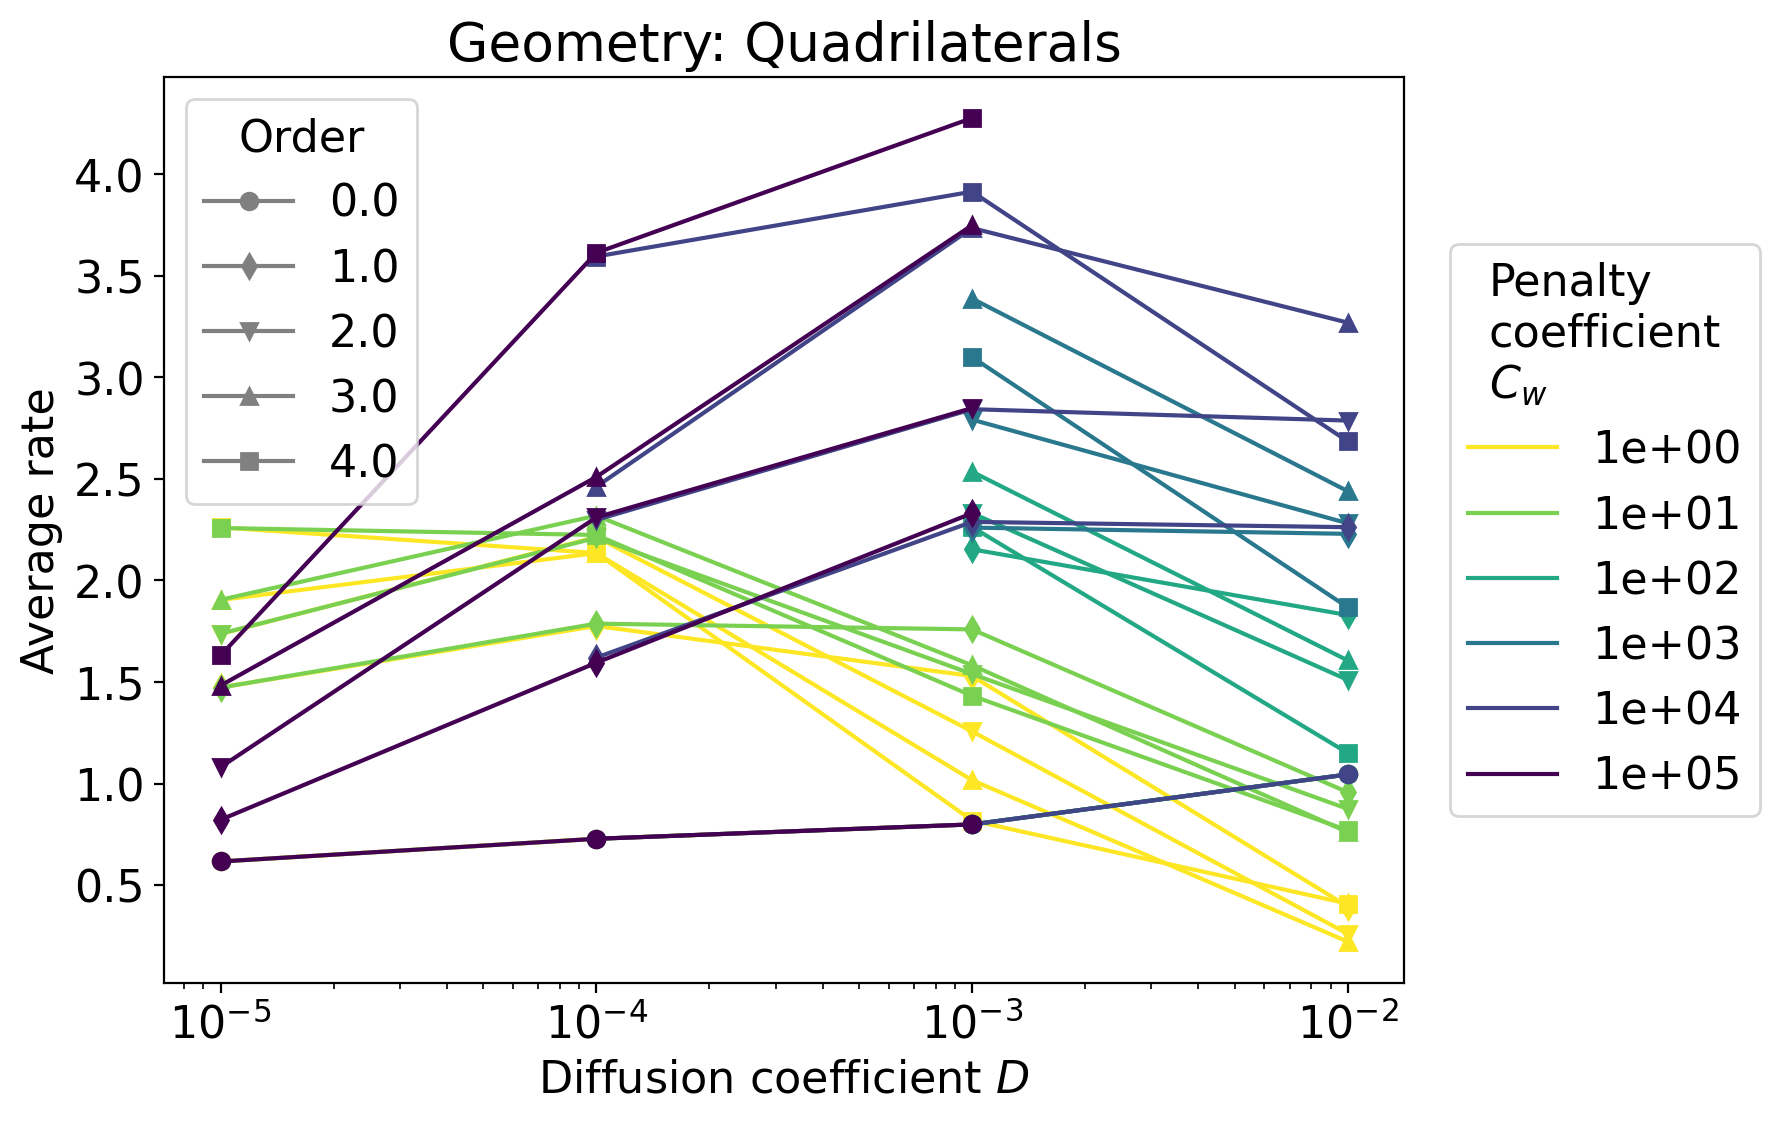
\includegraphics[width=0.49\textwidth]{../figs/parametric/advdiff_2D/ord_quarteroni2_2_4}
	&
	\vspace{0pt} 
	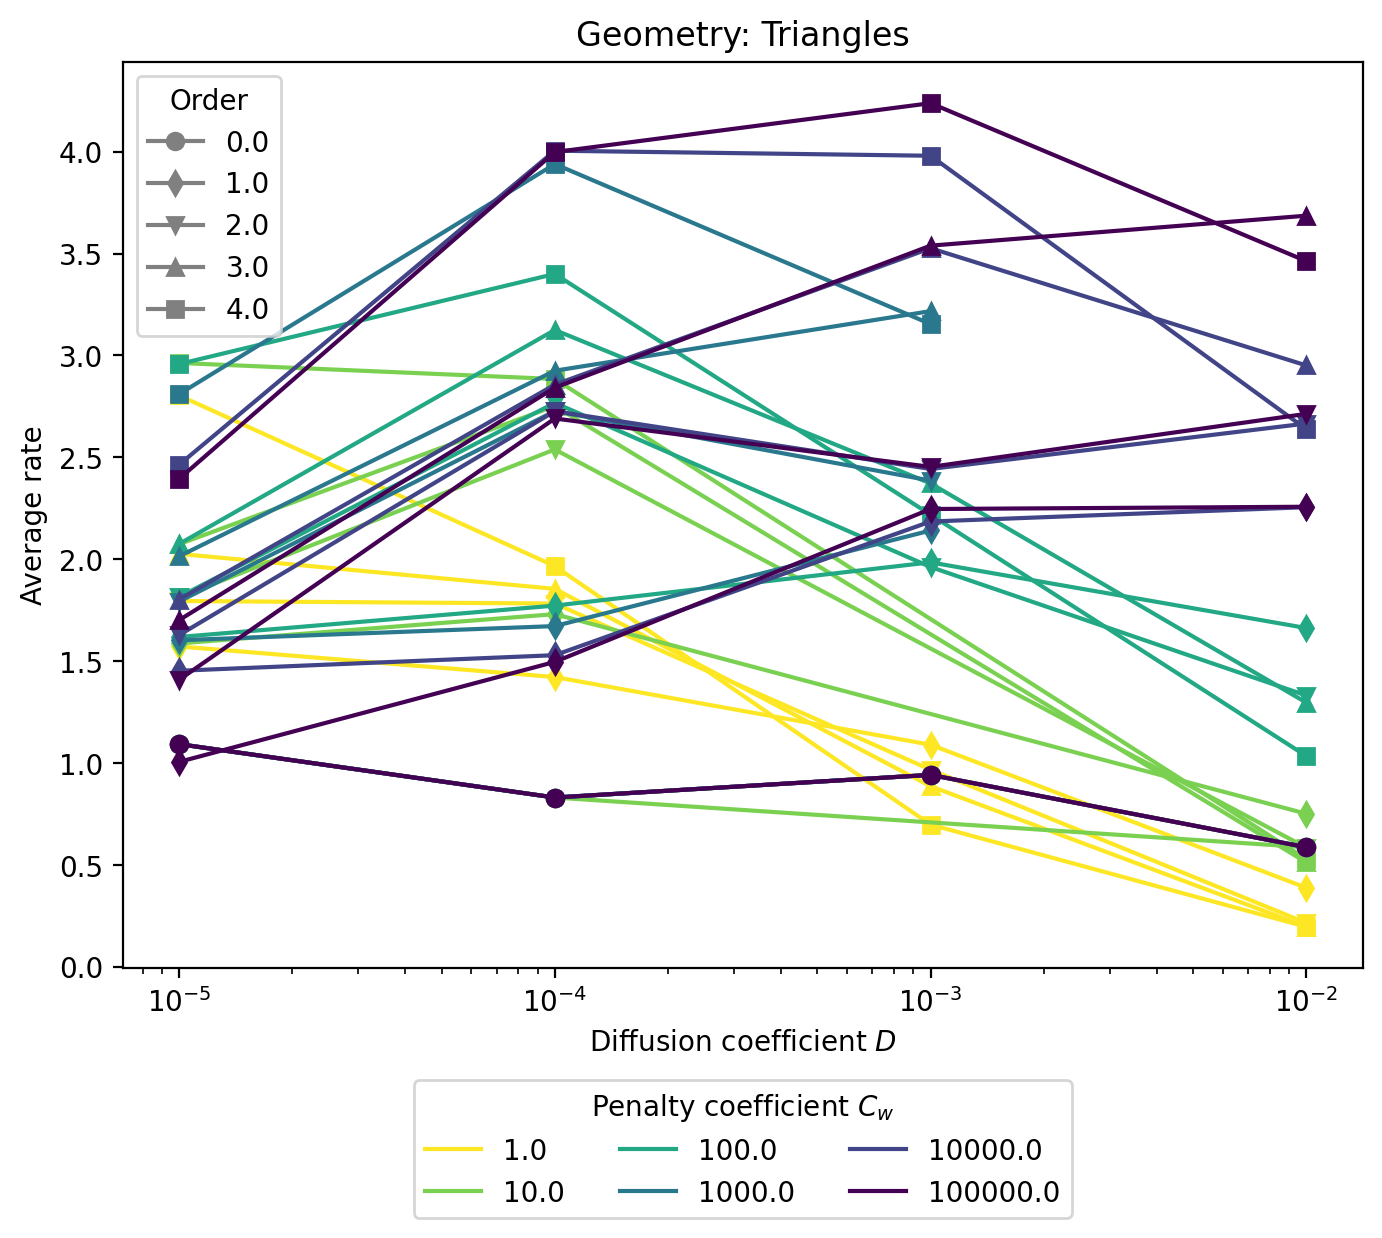
\includegraphics[width=0.49\textwidth]{../figs/parametric/advdiff_2D/ord_quarteroni2_2_3}
\end{tabular}
\caption{\Cref{ex:quart2} average order for different choice of $C_w$}
\label{fig:orders_quarteroni2}
\end{figure}


\begin{figure}[p!]
	\centering
	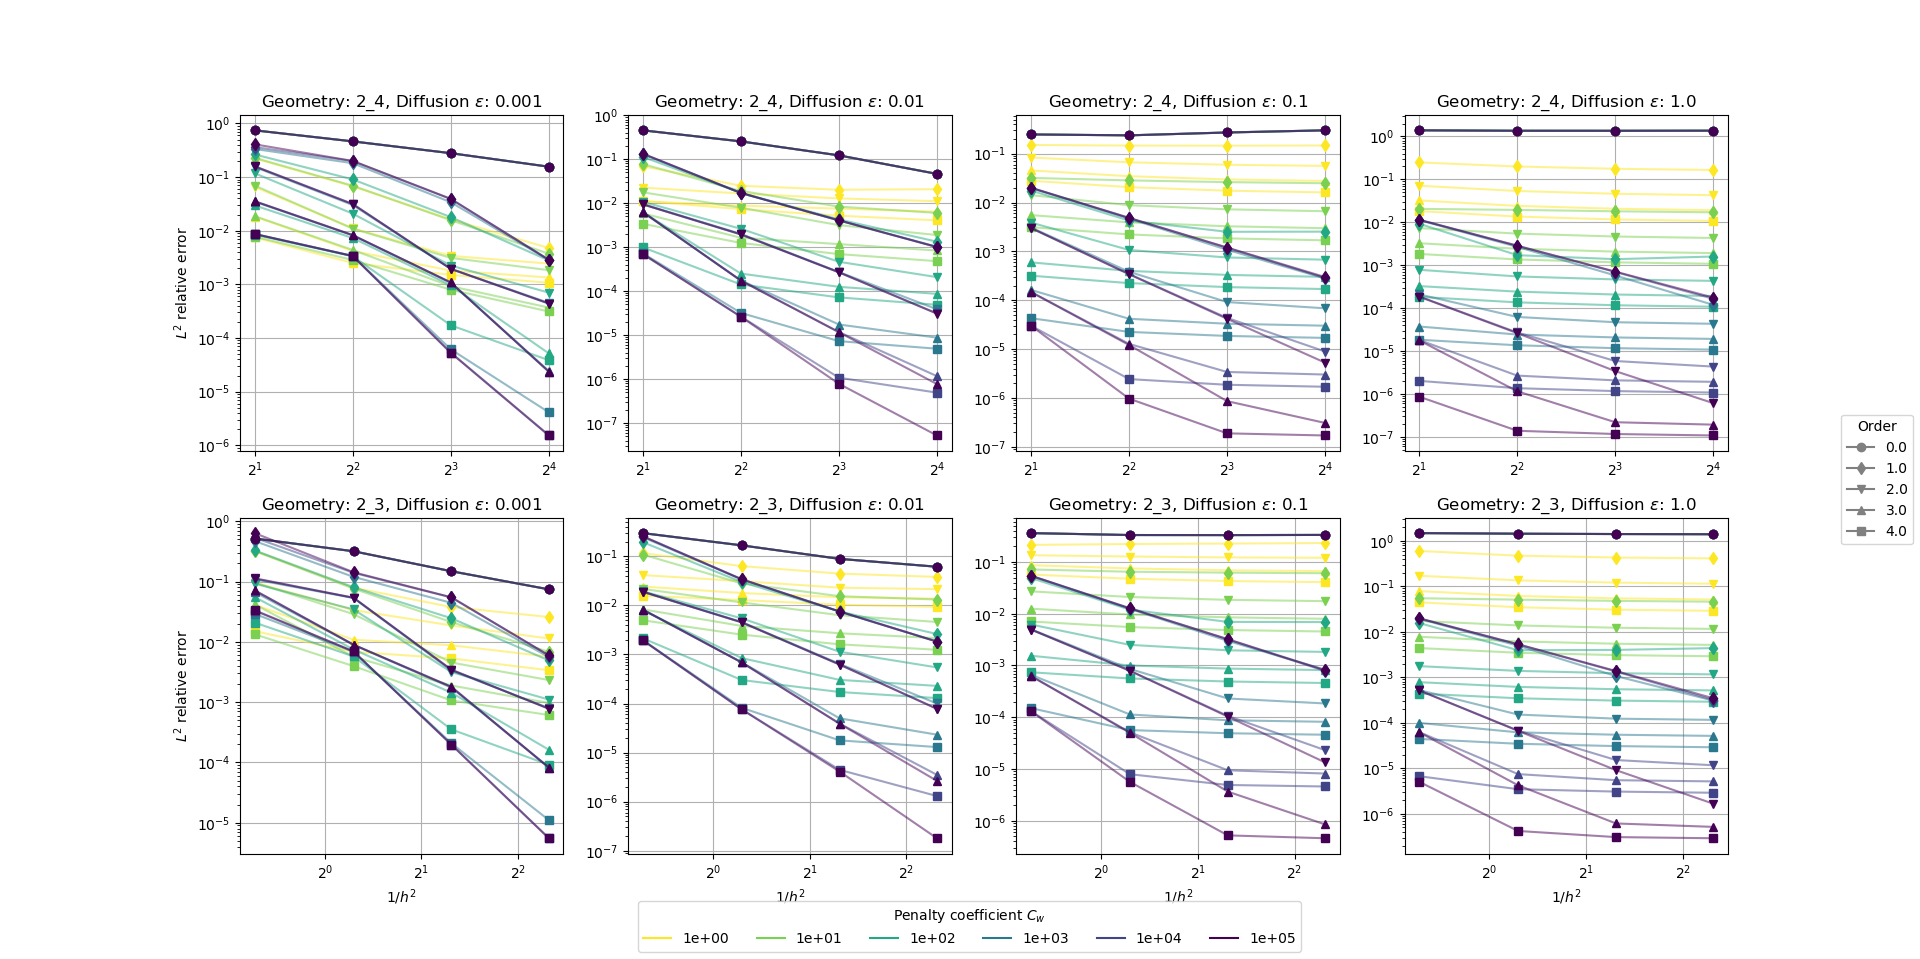
\includegraphics[height=\textheight]{../figs/parametric/advdiff_2D/quarteroni2}
	
	\caption{\Cref{ex:quart2} convergence graphs for different choice of $C_w$}
	\label{fig:conv_qart2}
\end{figure}
